\documentclass[beamer]{standalone}

\begin{document}
	\begin{frame}
		\color{blue}\centering\Huge{\textbf{Velocità Angolare}}	
	\end{frame}
	
	\begin{frame}{{Velocità Angolare}}
		\centering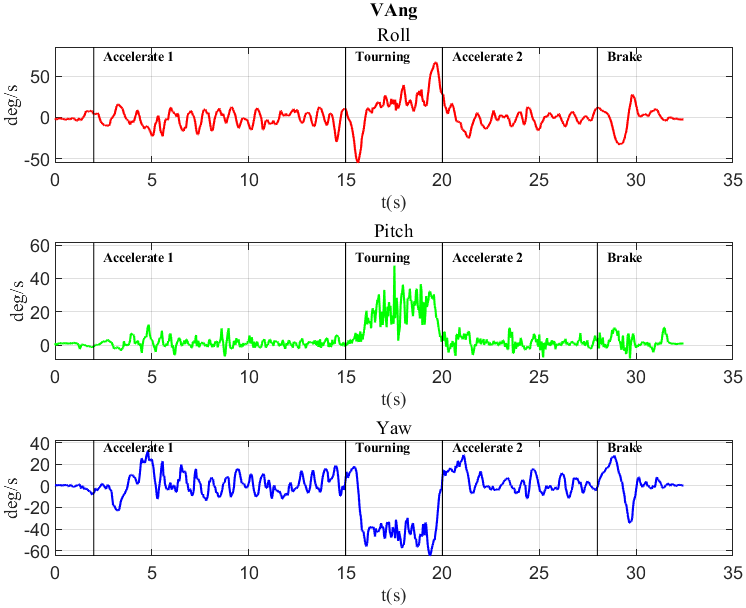
\includegraphics[height=.8\textheight]{figure/VAng/VAng}
	\end{frame}
	
	\begin{frame}{{Media}}
		\centering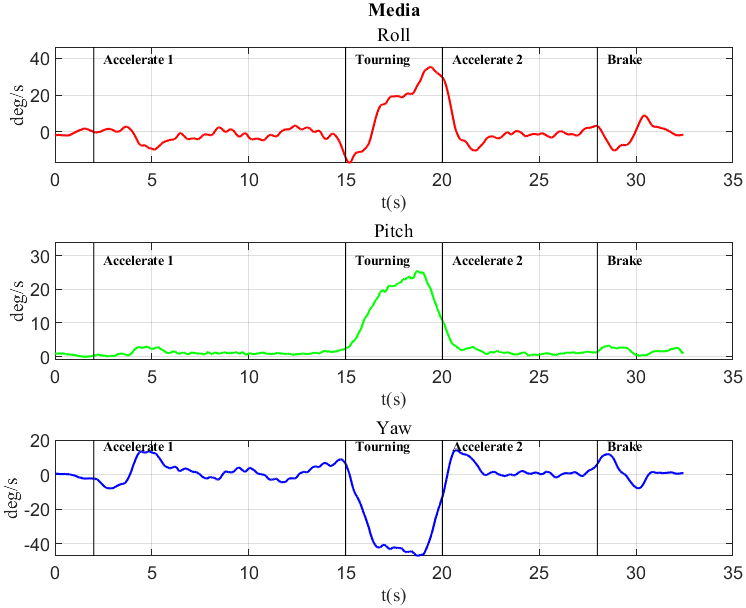
\includegraphics[height=.8\textheight]{figure/VAng/Media}
	\end{frame}
	
%	\begin{frame}{{Media Rettificata}}
%		\centering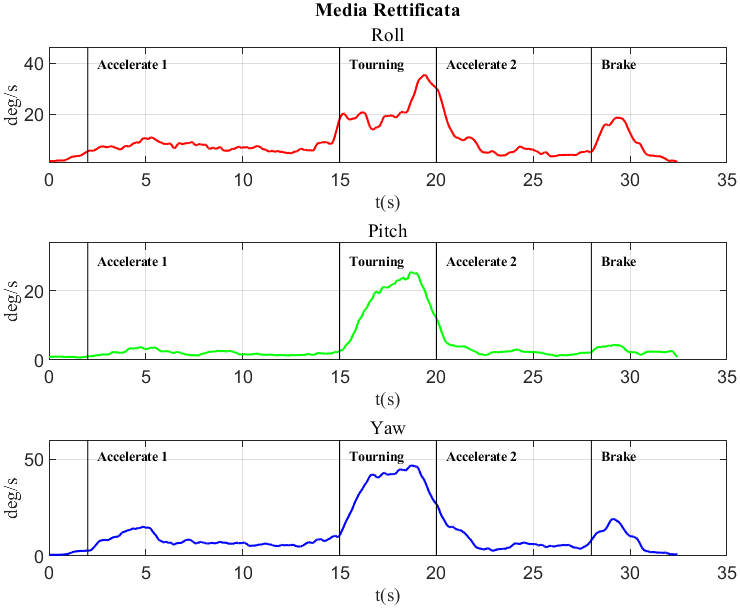
\includegraphics[height=.8\textheight]{figure/VAng/Media Rettificata}
%	\end{frame}
	
	\begin{frame}{{Varianza}}
		\centering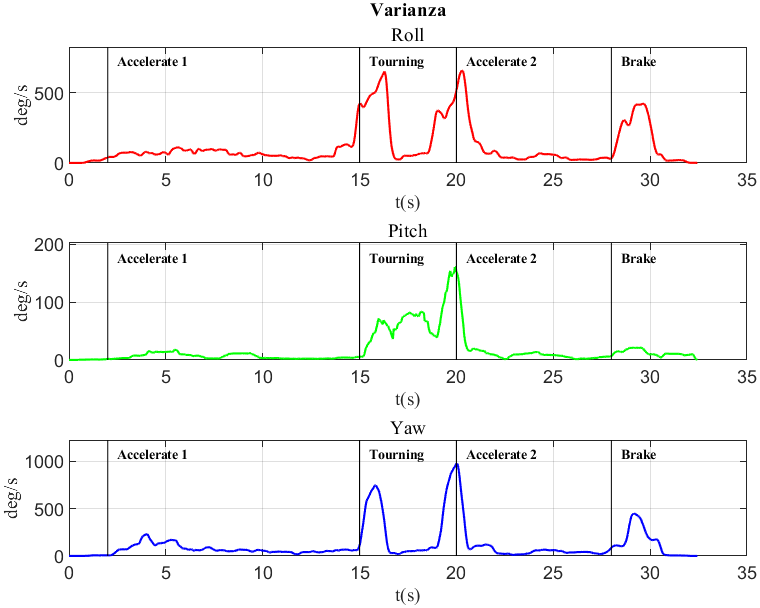
\includegraphics[height=.8\textheight]{figure/VAng/Varianza}
	\end{frame}
	
%	\begin{frame}{{Deviazione Standard}}
%		\centering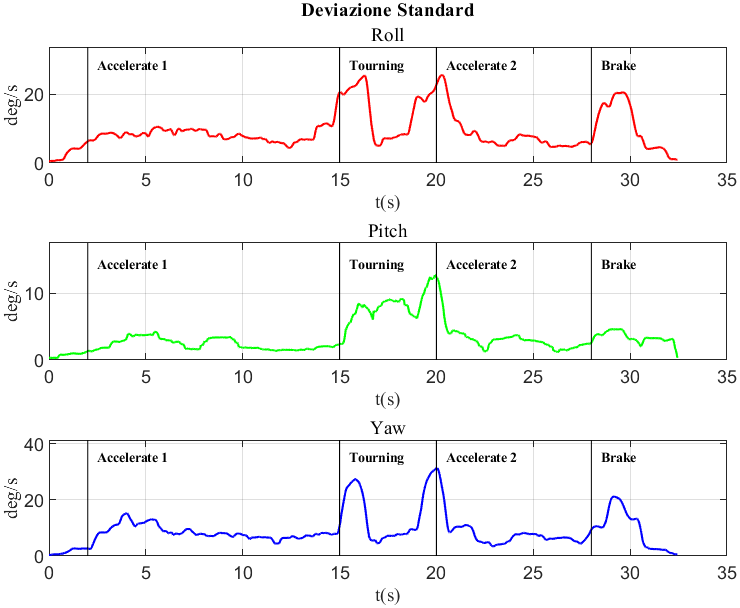
\includegraphics[height=.8\textheight]{figure/VAng/Deviazione Standard}
%	\end{frame}
	
%	\begin{frame}{{Scarto Quadratico Medio}}
%		\centering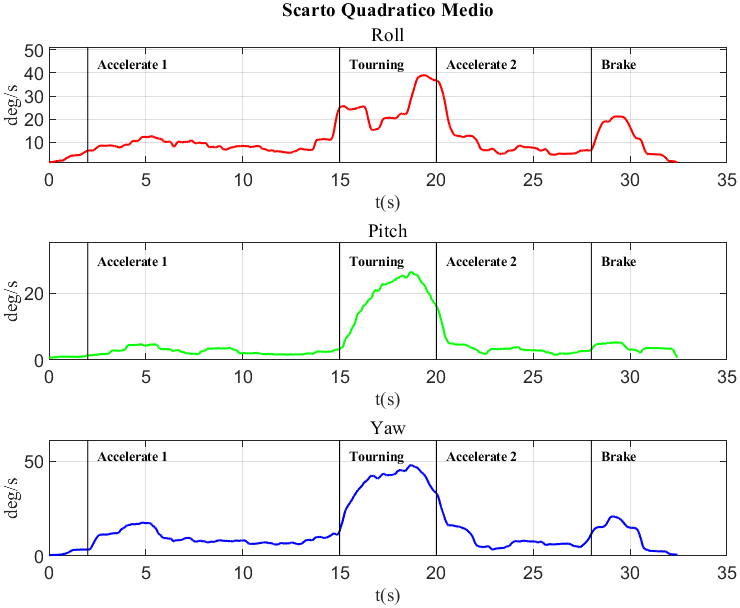
\includegraphics[height=.8\textheight]{figure/VAng/Scarto Quadratico Medio}
%	\end{frame}
	
%	\begin{frame}{{Max}}
%		\centering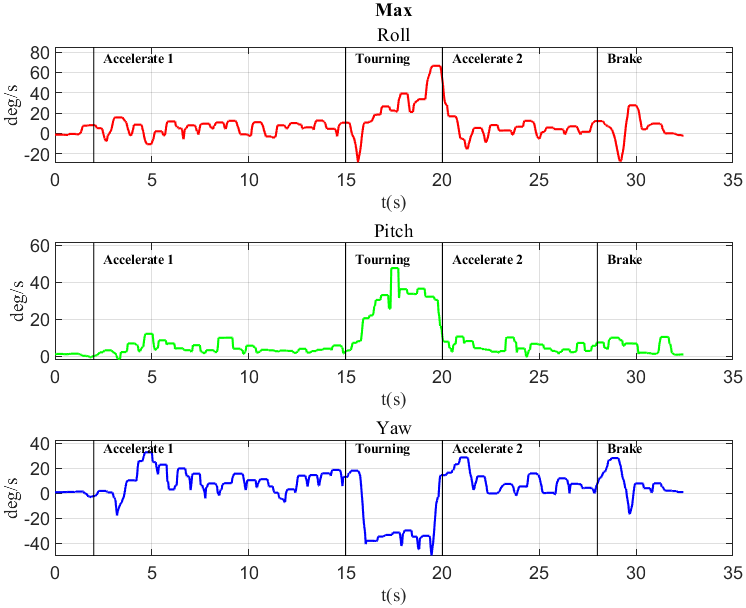
\includegraphics[height=.8\textheight]{figure/VAng/Max}
%	\end{frame}
%	
%	\begin{frame}{{Min}}
%		\centering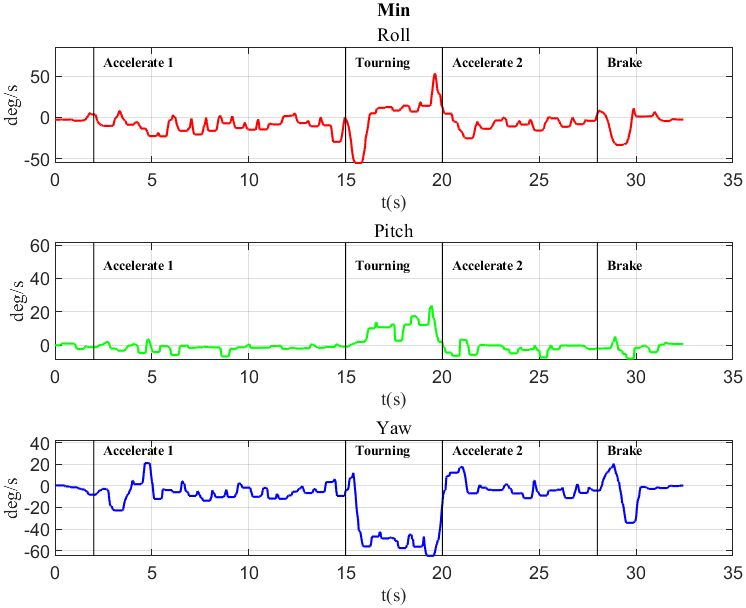
\includegraphics[height=.8\textheight]{figure/VAng/Min}
%	\end{frame}
%	
%	\begin{frame}{{Peak}}
%		\centering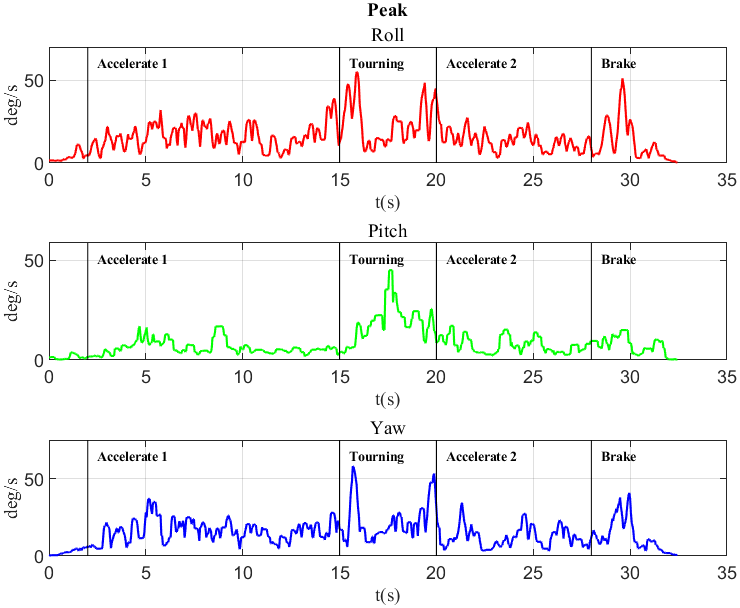
\includegraphics[height=.8\textheight]{figure/VAng/Peak}
%	\end{frame}
	
	\begin{frame}{{Kurtosi}}
		\centering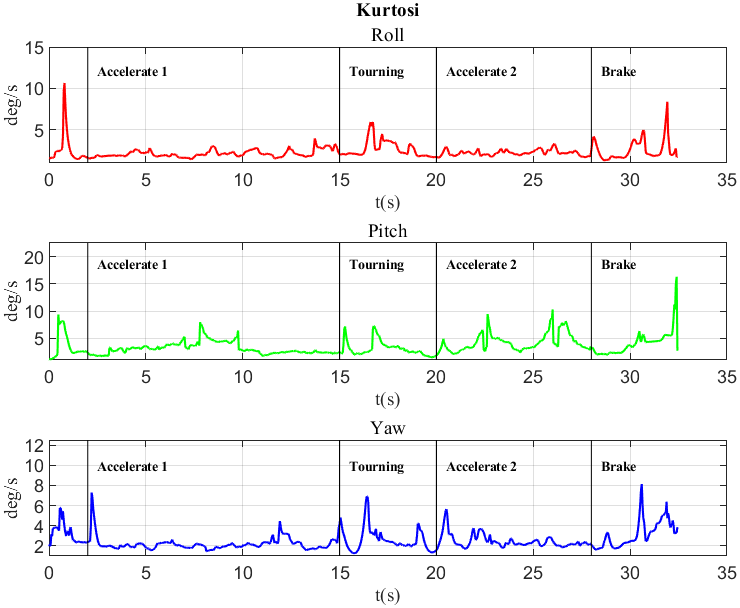
\includegraphics[height=.8\textheight]{figure/VAng/Kurtosi}
	\end{frame}
	
	\begin{frame}{{Skewness}}
		\centering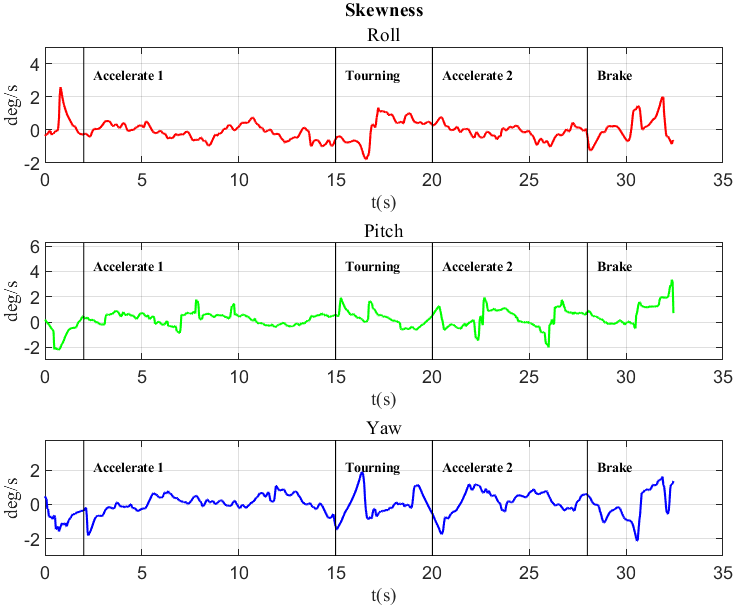
\includegraphics[height=.8\textheight]{figure/VAng/Skewness}
	\end{frame}
	
%	\begin{frame}{{Shape Factor}}
%		\centering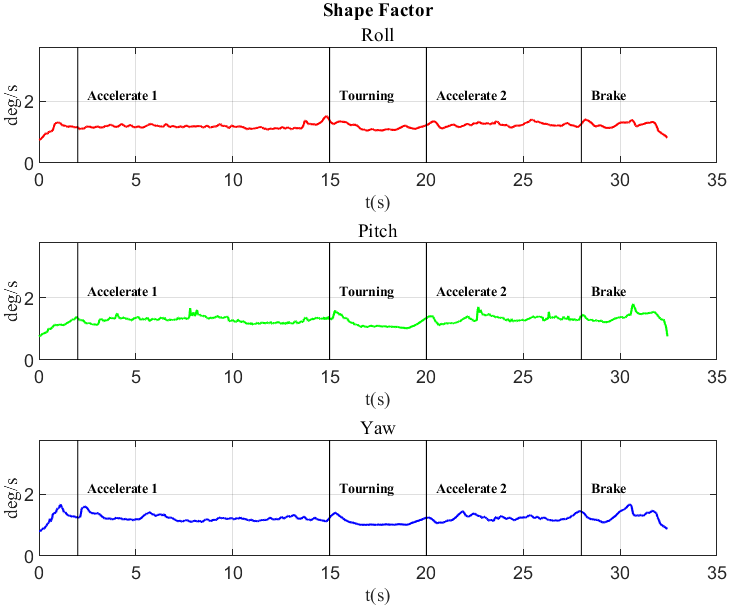
\includegraphics[height=.8\textheight]{figure/VAng/Shape Factor}
%	\end{frame}
	
	\begin{frame}{{Crest Factor}}
		\centering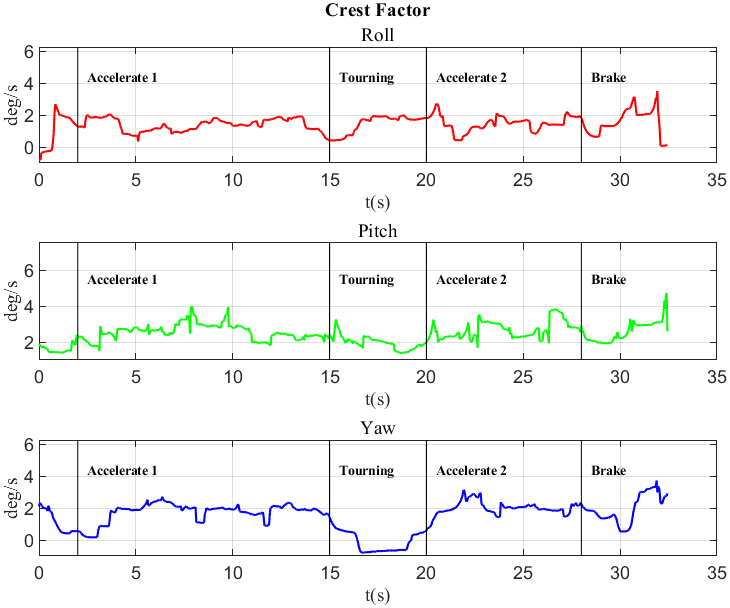
\includegraphics[height=.8\textheight]{figure/VAng/Crest Factor}
	\end{frame}
	
	\begin{frame}{{Impulse Factor}}
		\centering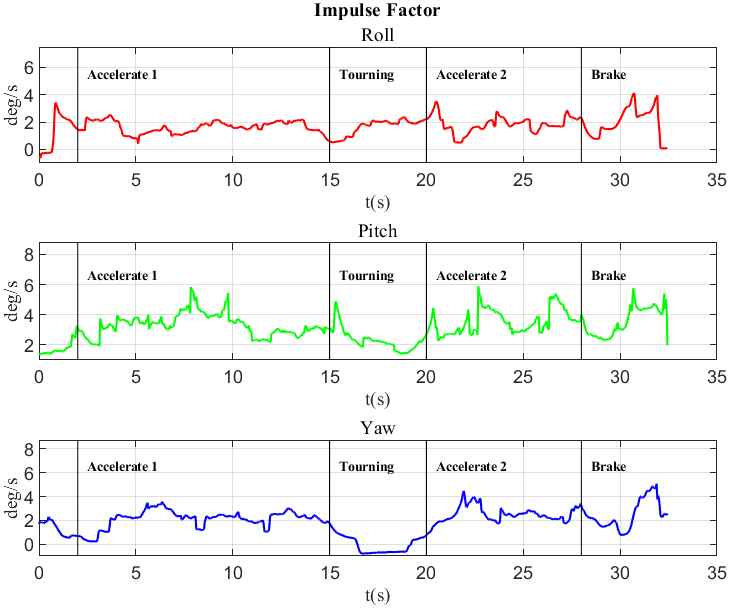
\includegraphics[height=.8\textheight]{figure/VAng/Impulse Factor}
	\end{frame}
	
	\begin{frame}{{Margin Factor}}
		\centering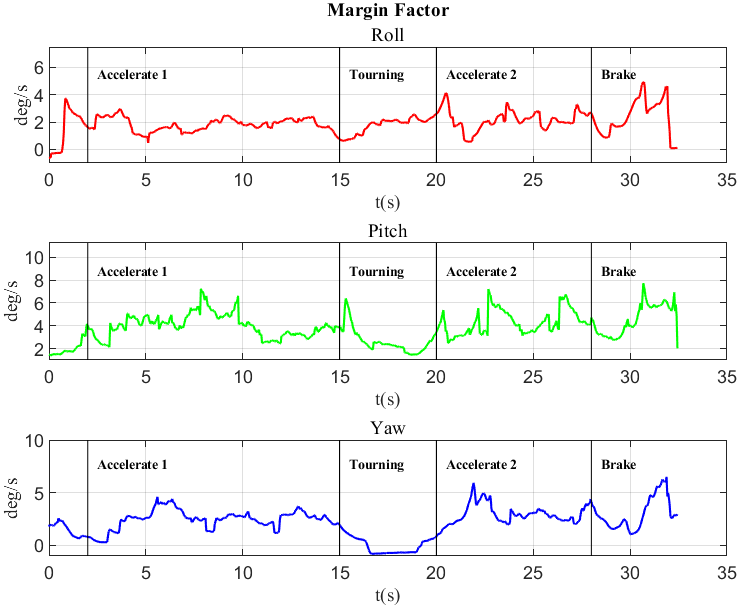
\includegraphics[height=.8\textheight]{figure/VAng/Margin Factor}
	\end{frame}
	
	\begin{frame}{{Trasformata}}
		\centering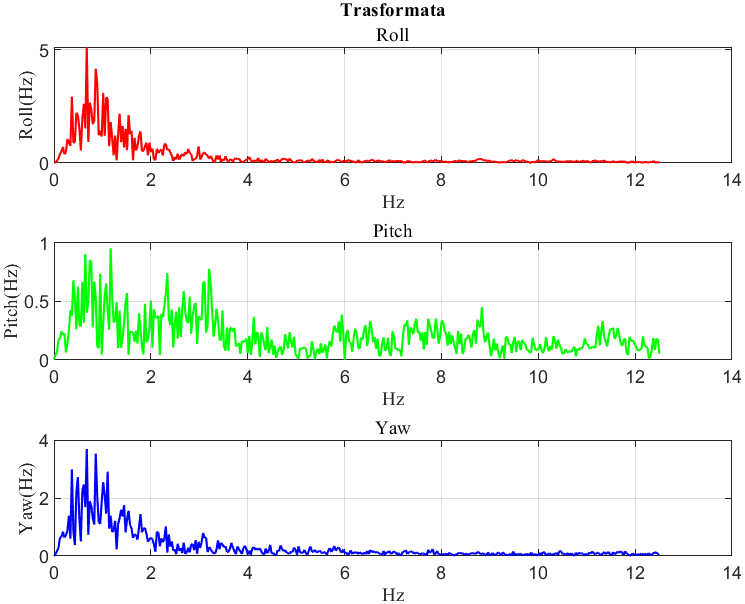
\includegraphics[height=.8\textheight]{figure/VAng/Trasformata/Trasformata}
	\end{frame}
	
	\begin{frame}{{Spettro}}
		\centering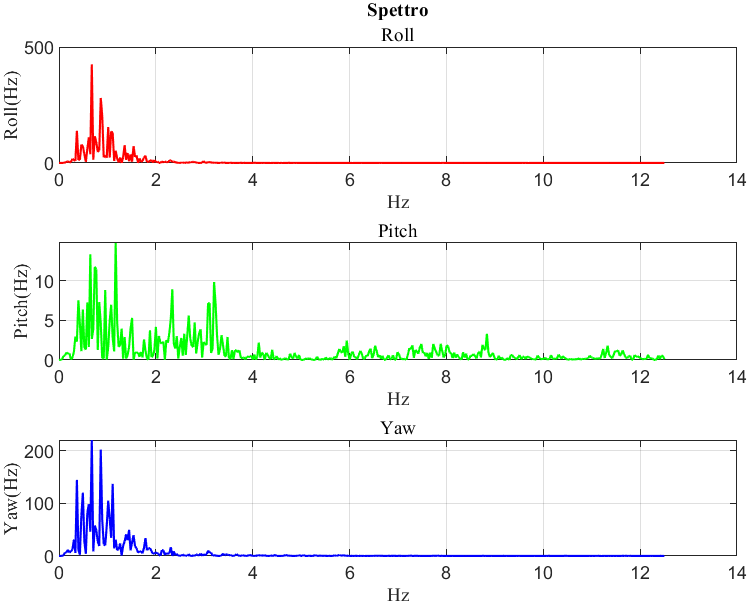
\includegraphics[height=.8\textheight]{figure/VAng/Trasformata/Spettro}
	\end{frame}
	
	\begin{frame}
		\color{blue}\centering\huge{\textbf{Trasformata Velocità Angolare}}
	\end{frame}
	
	\begin{frame}{{Trasformata Accelerazione 1}}
		\centering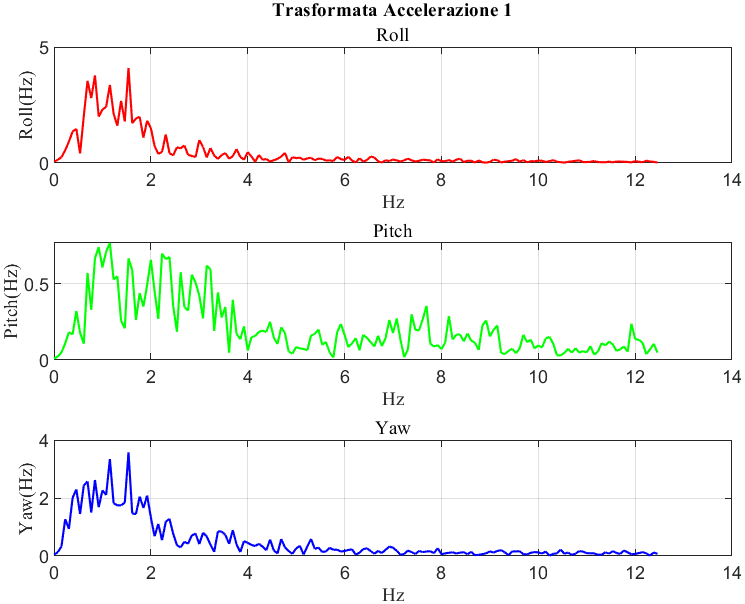
\includegraphics[height=.8\textheight]{figure/VAng/Trasformata/Trasformata Accelerazione 1}
	\end{frame}
	
	\begin{frame}{{Trasformata Tourning}}
		\centering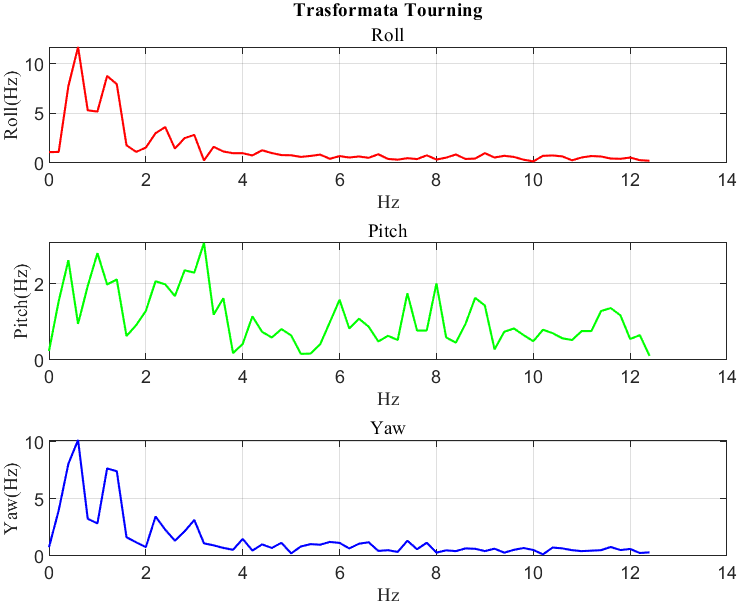
\includegraphics[height=.8\textheight]{figure/VAng/Trasformata/Trasformata Tourning}
	\end{frame}
	
	\begin{frame}{{Trasformata Accelerazione 2}}
		\centering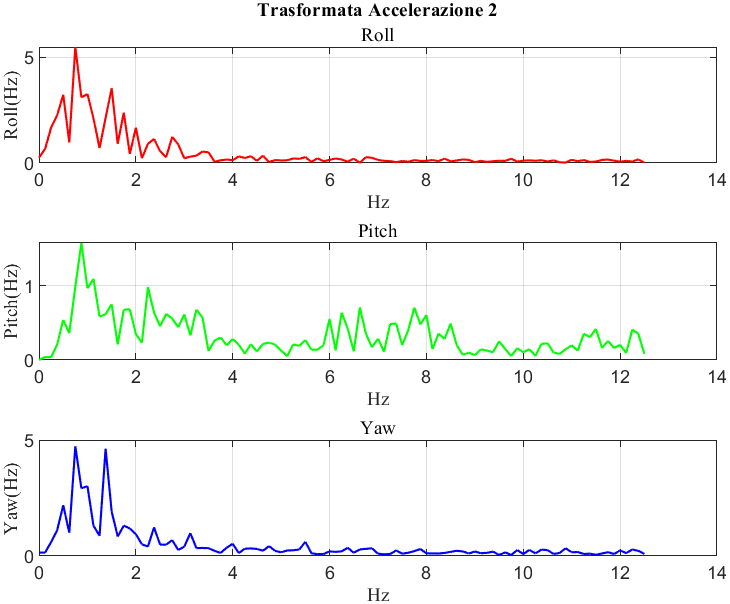
\includegraphics[height=.8\textheight]{figure/VAng/Trasformata/Trasformata Accelerazione 2}
	\end{frame}
	
	\begin{frame}{{Trasformata Brake}}
		\centering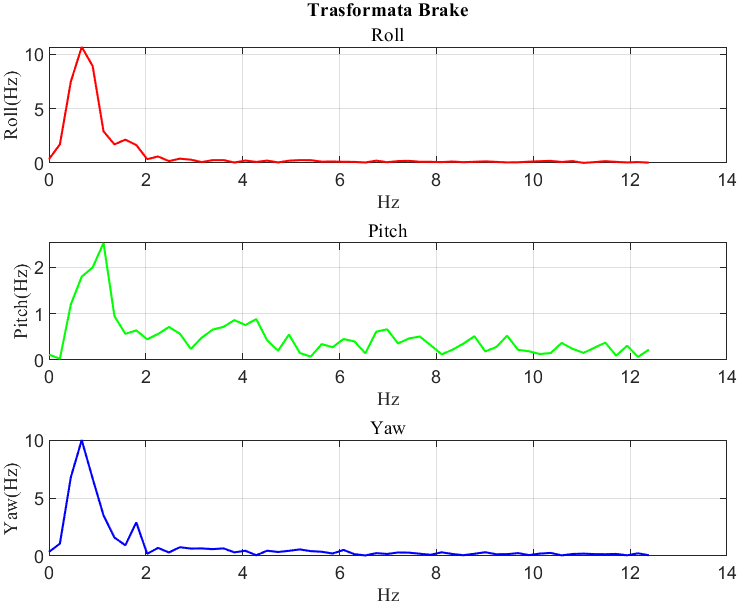
\includegraphics[height=.8\textheight]{figure/VAng/Trasformata/Trasformata Brake}
	\end{frame}
	
	\begin{frame}{{Ampiezza Media Roll}}
		\centering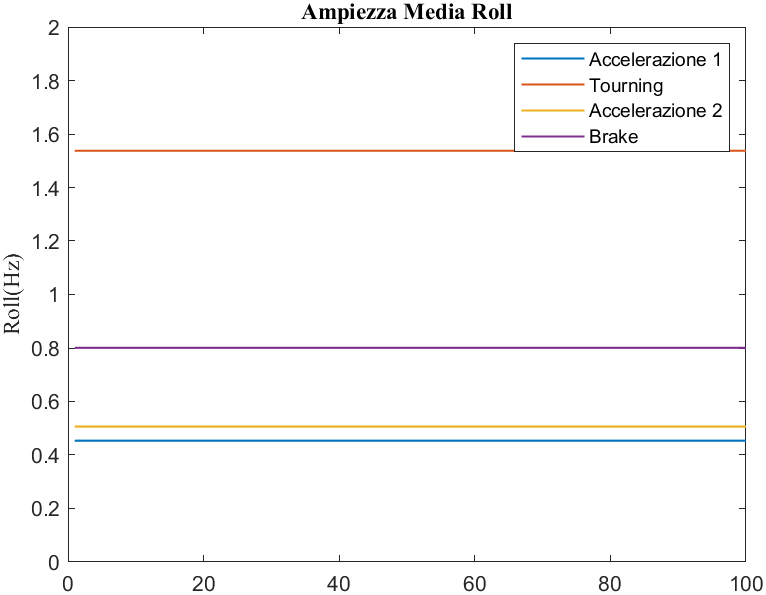
\includegraphics[height=.8\textheight]{figure/VAng/Trasformata/Ampiezza MediaRoll}
	\end{frame}
	
	\begin{frame}{{Ampiezza Media Pitch}}
		\centering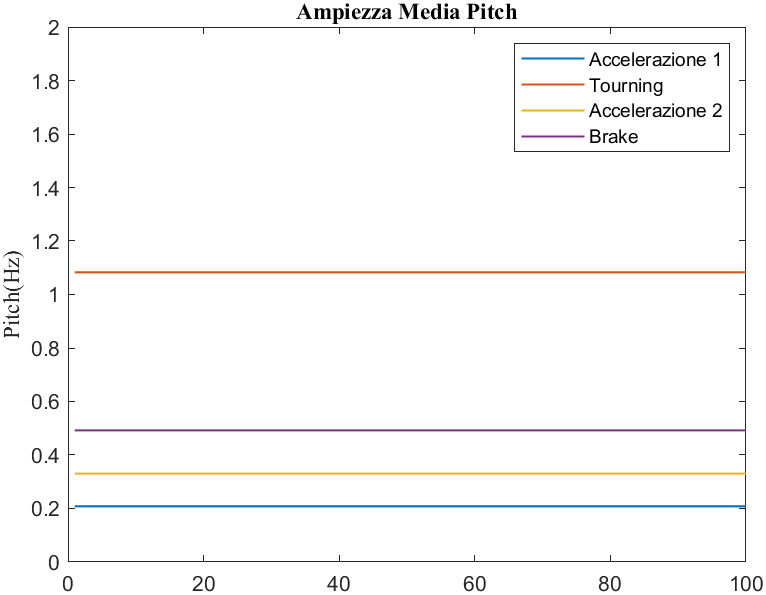
\includegraphics[height=.8\textheight]{figure/VAng/Trasformata/Ampiezza MediaPitch}
	\end{frame}
	
	\begin{frame}{{Ampiezza Media Yaw}}
		\centering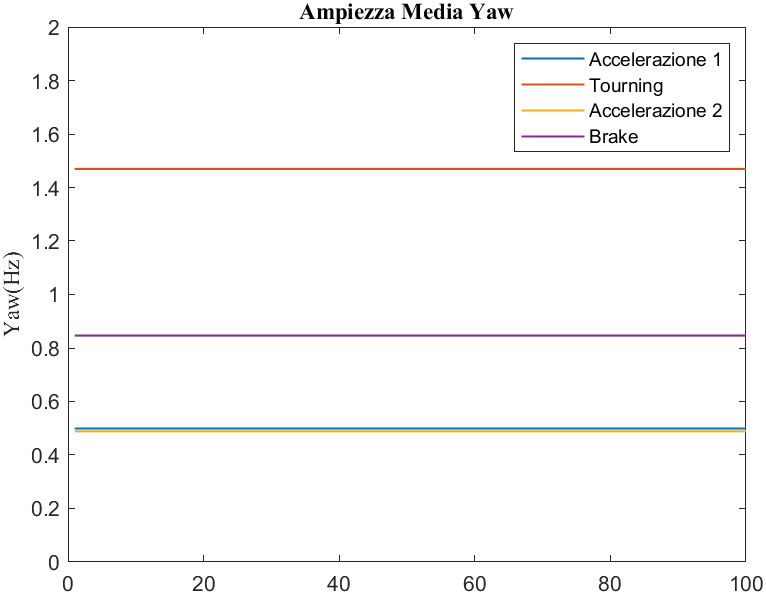
\includegraphics[height=.8\textheight]{figure/VAng/Trasformata/Ampiezza MediaYaw}
	\end{frame}
	
	\begin{frame}{{Frequency Centroid Roll}}
		\centering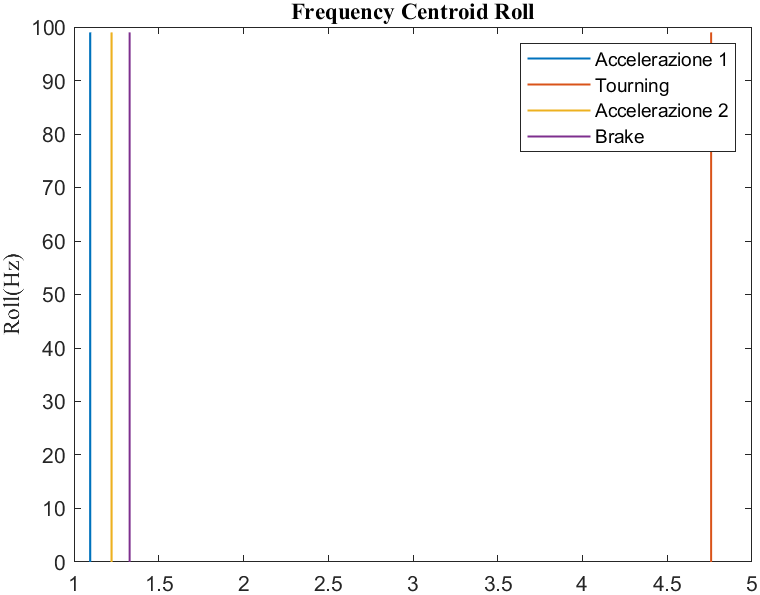
\includegraphics[height=.8\textheight]{figure/VAng/Trasformata/Frequency CentroidRoll}
	\end{frame}
	
	\begin{frame}{{Frequency Centroid Pitch}}
		\centering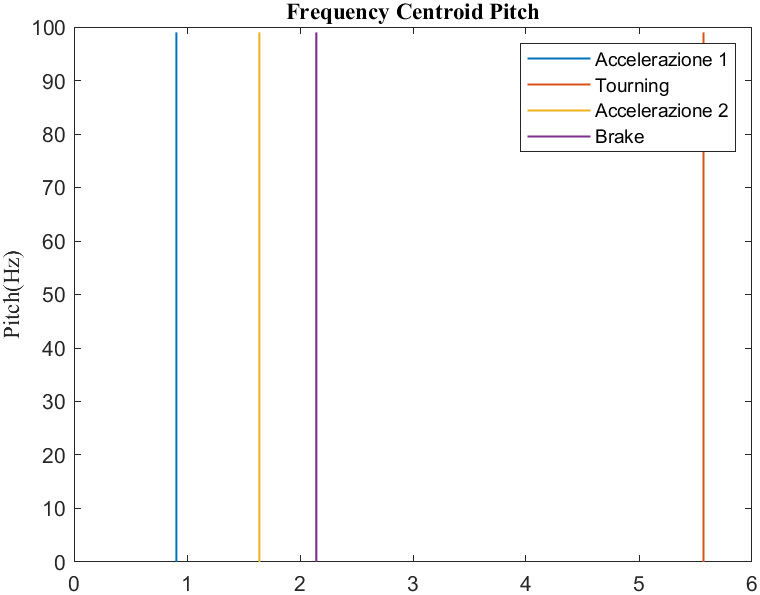
\includegraphics[height=.8\textheight]{figure/VAng/Trasformata/Frequency CentroidPitch}
	\end{frame}
	
	\begin{frame}{{Frequency Centroid Yaw}}
		\centering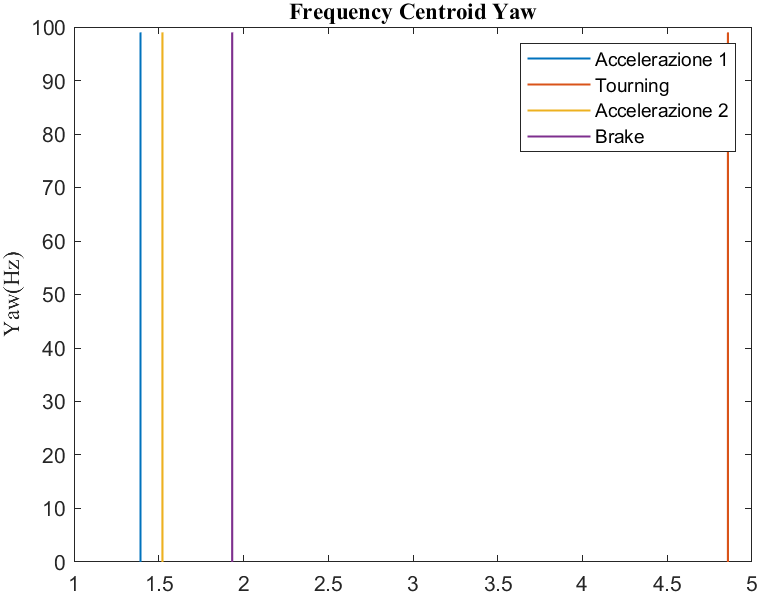
\includegraphics[height=.8\textheight]{figure/VAng/Trasformata/Frequency CentroidYaw}
	\end{frame}
	
	\begin{frame}{{Frequency Variance Roll}}
		\centering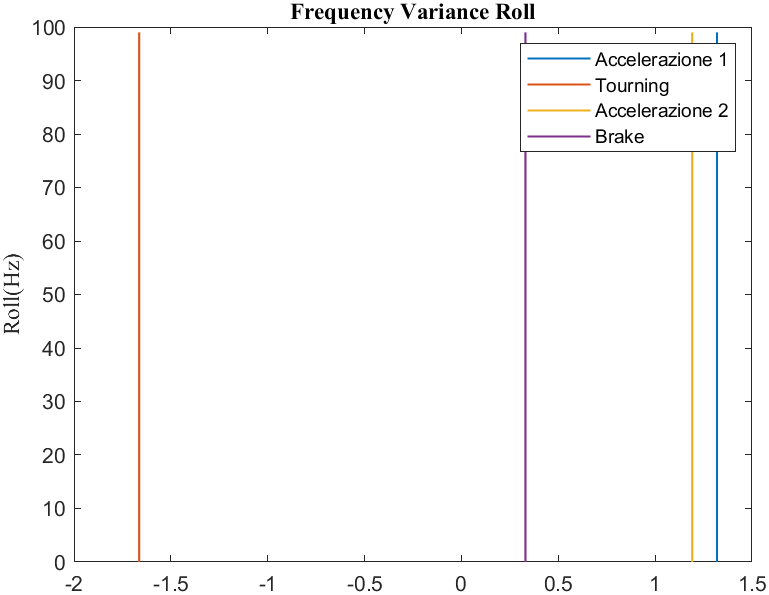
\includegraphics[height=.8\textheight]{figure/VAng/Trasformata/Frequency VarianceRoll}
	\end{frame}
	
	\begin{frame}{{Frequency Variance Pitch}}
		\centering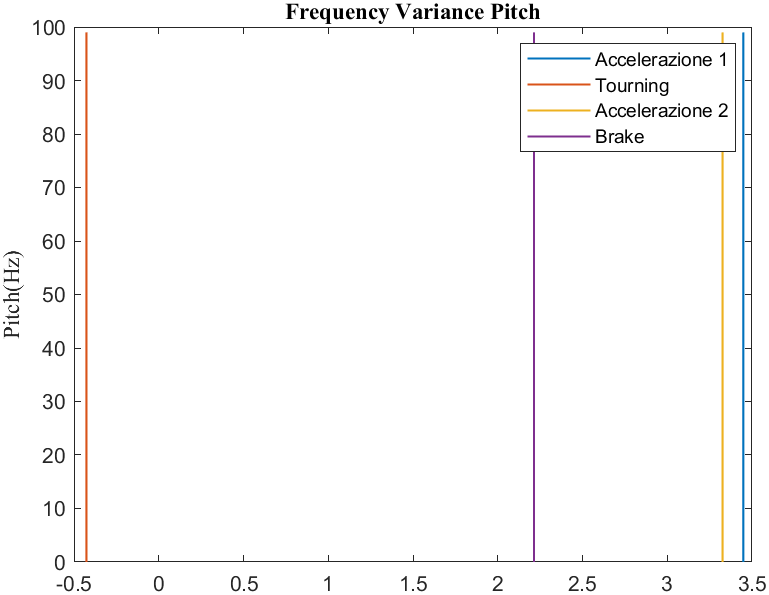
\includegraphics[height=.8\textheight]{figure/VAng/Trasformata/Frequency VariancePitch}
	\end{frame}
	
	\begin{frame}{{Frequency Variance Yaw}}
		\centering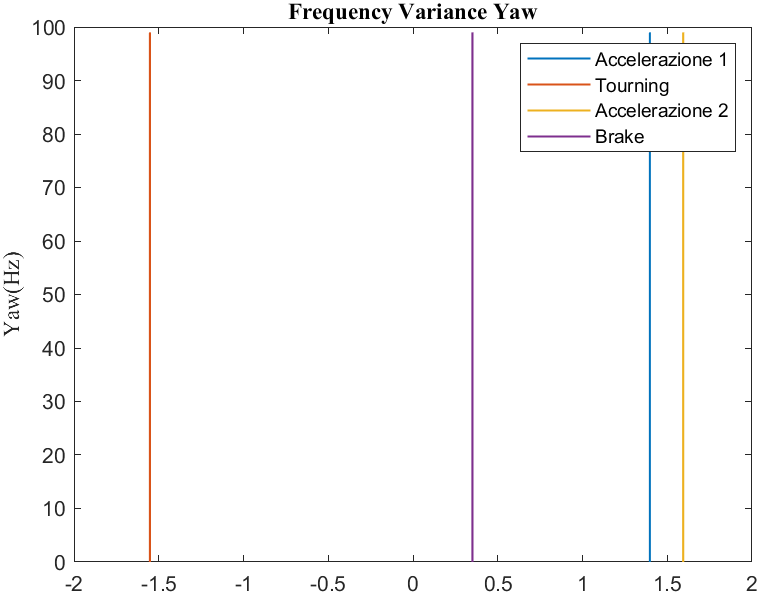
\includegraphics[height=.8\textheight]{figure/VAng/Trasformata/Frequency VarianceYaw}
	\end{frame}
	
	\begin{frame}
		\color{blue}\centering\huge{\textbf{Spettro Velocità Angolare}}
	\end{frame}
	
	\begin{frame}{{Spettro Accelerazione 1}}
		\centering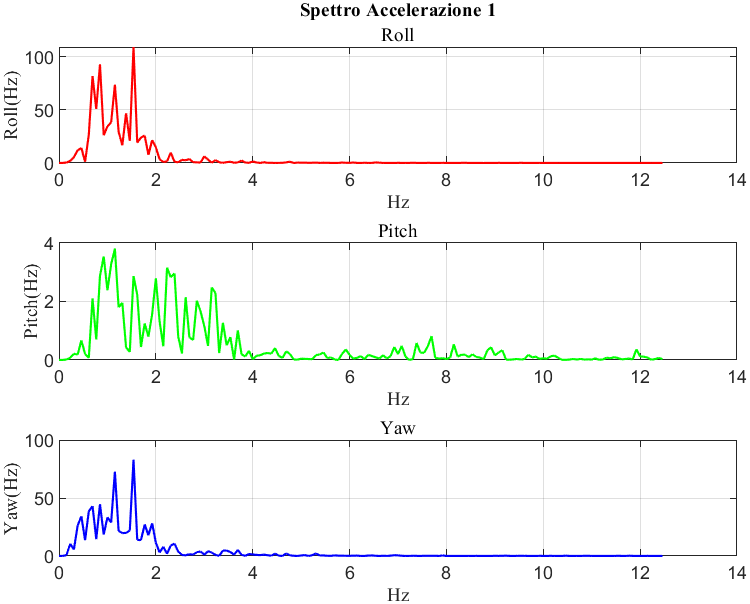
\includegraphics[height=.8\textheight]{figure/VAng/Trasformata/Spettro Accelerazione 1}
	\end{frame}
	
	\begin{frame}{{Spettro Tourning}}
		\centering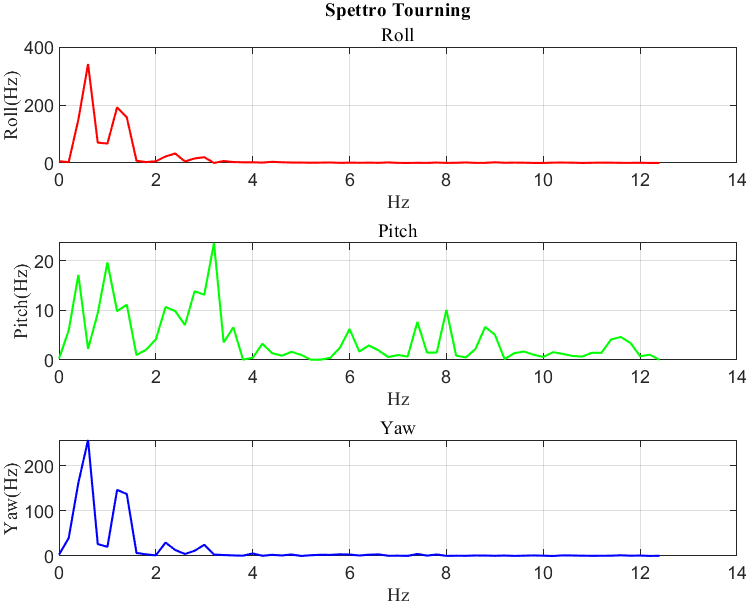
\includegraphics[height=.8\textheight]{figure/VAng/Trasformata/Spettro Tourning}
	\end{frame}
	
	\begin{frame}{{Spettro Accelerazione 2}}
		\centering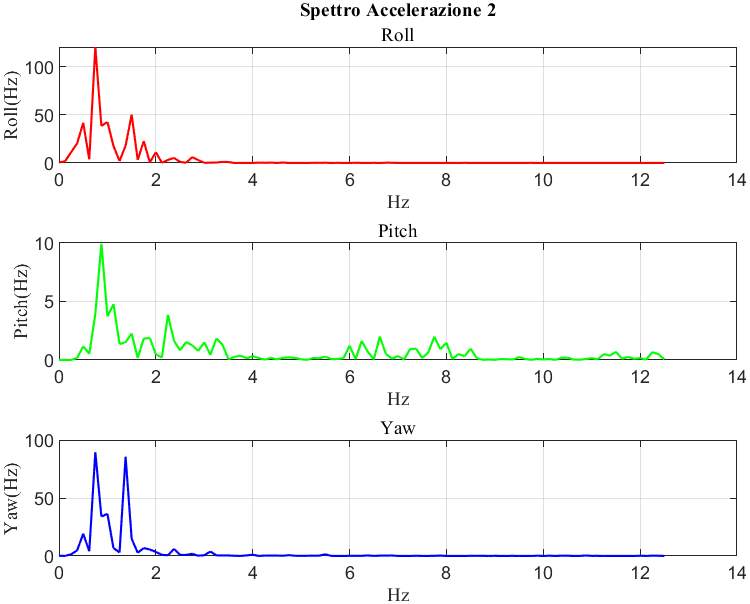
\includegraphics[height=.8\textheight]{figure/VAng/Trasformata/Spettro Accelerazione 2}
	\end{frame}
	
	\begin{frame}{{Spettro Brake}}
		\centering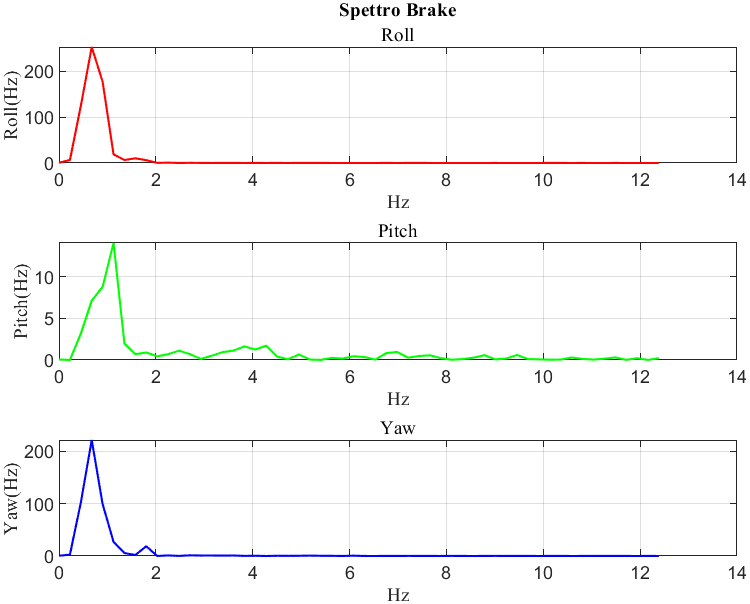
\includegraphics[height=.8\textheight]{figure/VAng/Trasformata/Spettro Brake}
	\end{frame}
	
	\begin{frame}{{Spectral Entropy Roll}}
		\centering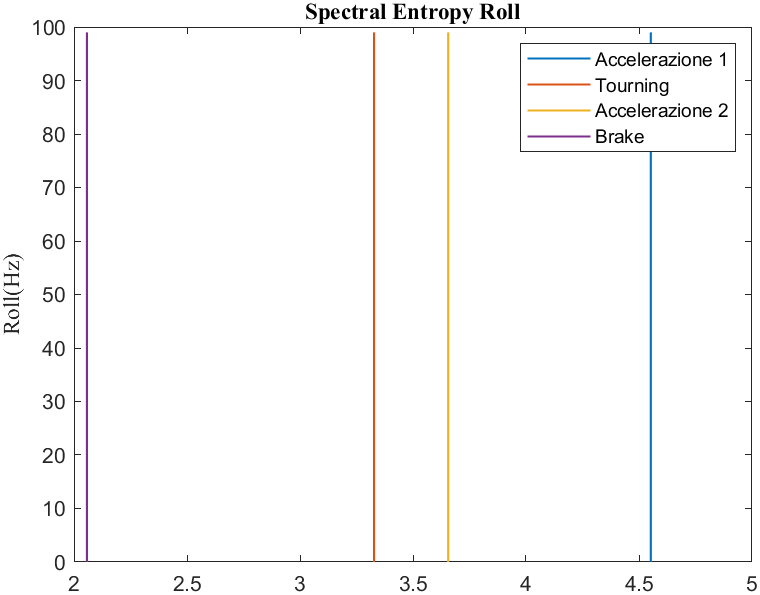
\includegraphics[height=.8\textheight]{figure/VAng/Trasformata/Spectral EntropyRoll}
	\end{frame}
	
	\begin{frame}{{Spectral Entropy Pitch}}
		\centering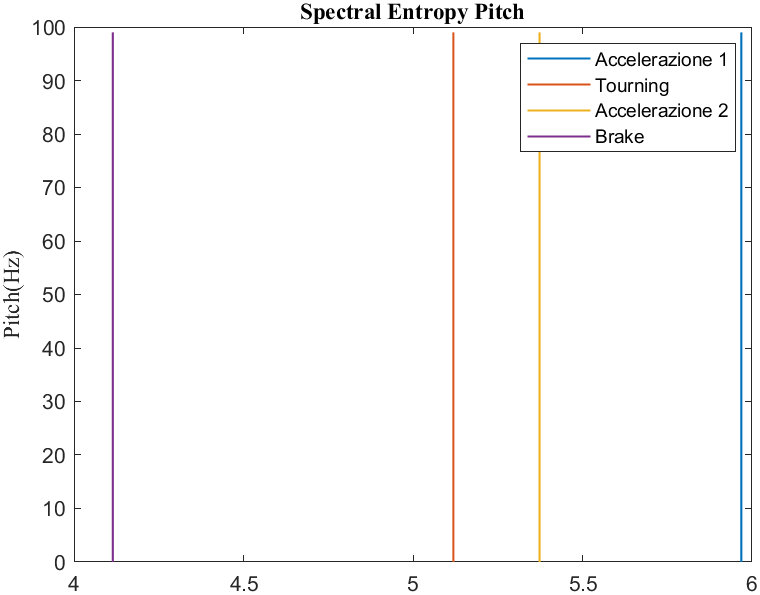
\includegraphics[height=.8\textheight]{figure/VAng/Trasformata/Spectral EntropyPitch}
	\end{frame}
	
	\begin{frame}{{Spectral Entropy Yaw}}
		\centering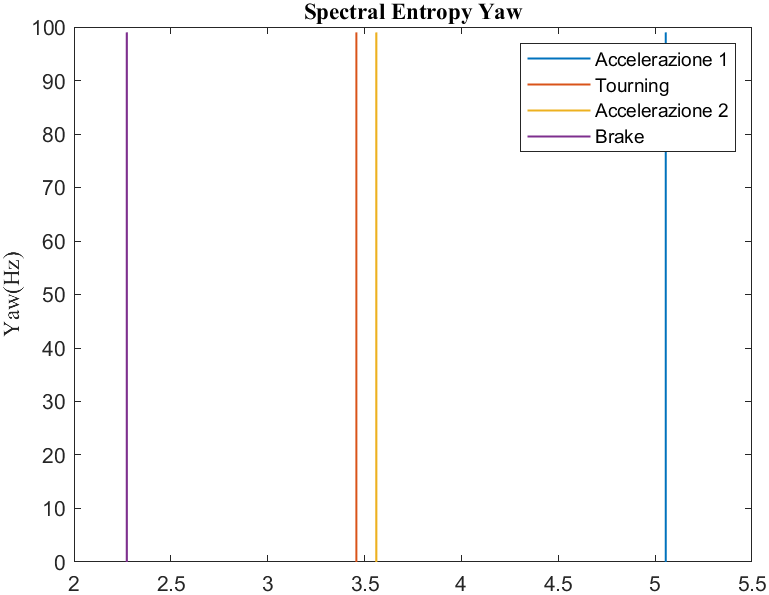
\includegraphics[height=.8\textheight]{figure/VAng/Trasformata/Spectral EntropyYaw}
	\end{frame}
	
\end{document}